\documentclass[8pt,executivepaper]{article}
\usepackage[utf8]{inputenc}
\usepackage[spanish]{babel}
\usepackage{amsmath}
\usepackage{amsfonts}
\usepackage{amssymb}
\usepackage{graphics}
\usepackage{graphicx}
\usepackage[left=1cm,right=1cm,top=2cm,bottom=2cm]{geometry}
\usepackage{imakeidx}
\makeindex[columns=3, title=Alphabetical Index, intoc]
\usepackage{listings}
\usepackage{xcolor}
\usepackage{multicol}
\usepackage{changepage}
\usepackage{float}
\usepackage{cite}
\usepackage{url}
\usepackage{hyperref}
\usepackage{pdfpages}
\usepackage{pgf,pgffor}

\definecolor{codegreen}{rgb}{0,0.6,0}
\definecolor{codegray}{rgb}{0.5,0.5,0.5}
\definecolor{codepurple}{rgb}{0.58,0,0.82}
\definecolor{backcolour}{rgb}{0.95,0.95,0.92}
\lstdefinestyle{mystyle}{
    backgroundcolor=\color{backcolour},
    commentstyle=\color{codegreen},
    keywordstyle=\color{magenta},
    numberstyle=\tiny\color{codegray},
    stringstyle=\color{codepurple},
    basicstyle=\ttfamily\footnotesize,
    breakatwhitespace=false,
    breaklines=true,
    captionpos=b,
    keepspaces=true,
    numbers=left,
    numbersep=5pt,
    showspaces=false,
    showstringspaces=false,
    showtabs=false,
    tabsize=3
}
\lstset{style=mystyle}
\author{González Pardo Adrian}
\date{Junio 2020}
\title{Reporte de practica 14}
\newcommand\tab[1][1cm]{\hspace*{#1}}
\begin{document}
\maketitle

\section{Código fuente de los componentes:}
\subsection{Registro}
\begin{center}
  \lstinputlisting[language=VHDL]{vhd/registro.vhd}
\end{center}
\subsection{Bloque de condición}
\begin{center}
  \lstinputlisting[language=VHDL]{vhd/condition.vhd}
\end{center}
\subsection{Bloque decodificador}
\begin{center}
  \lstinputlisting[language=VHDL]{vhd/decInstrucciones.vhd}
\end{center}
\subsection{Bloque de nivel}
\begin{center}
  \lstinputlisting[language=VHDL]{vhd/level.vhd}
\end{center}
\subsection{MFunCode}
\begin{center}
  \lstinputlisting[language=VHDL]{vhd/mfuncode.vhd}
\end{center}
\subsection{MOpCode}
\begin{center}
  \lstinputlisting[language=VHDL]{vhd/mopcode.vhd}
\end{center}
\subsection{Unidad de Control}
\begin{center}
  \lstinputlisting[language=VHDL]{vhd/unControl.vhd}
\end{center}

\section{Código fuente del empaquetado}
\begin{center}
  \lstinputlisting[language=VHDL]{vhd/paqueteHardware.vhd}
\end{center}
\section{Código fuente de la unión para la arquitectura completa}
\begin{center}
  \lstinputlisting[language=VHDL]{vhd/arquitectura.vhd}
\end{center}

\section{Test-Bench:}
\subsection{Registro}
\begin{center}
  \lstinputlisting[language=VHDL]{tb/registro_TB.vhd}
\end{center}
\subsection{Bloque de condición}
\begin{center}
  \lstinputlisting[language=VHDL]{tb/condition_TB.vhd}
\end{center}
\subsection{Bloque decodificador}
\begin{center}
  \lstinputlisting[language=VHDL]{tb/decodificador_TB.vhd}
\end{center}
\subsection{Bloque de nivel}
\begin{center}
  \lstinputlisting[language=VHDL]{tb/level_TB.vhd}
\end{center}
\subsection{MFunCode}
\begin{center}
  \lstinputlisting[language=VHDL]{tb/mfuncode_TB.vhd}
\end{center}
\subsection{MOpCode}
\begin{center}
  \lstinputlisting[language=VHDL]{tb/mopcode_TB.vhd}
\end{center}
\subsection{Unidad de Control}
\begin{center}
  \lstinputlisting[language=VHDL]{tb/unControl_TB.vhd}
\end{center}
\subsection{Arquitectura completa}
\begin{center}
  \lstinputlisting[language=VHDL]{tb/arquitectura_TB.vhd}
\end{center}

\section{Archivos de texto input/output}
\subsection{Entrada}
\begin{center}
  \lstinputlisting{in.txt}
\end{center}
\subsection{Salida}
\begin{center}
  \lstinputlisting{out.txt}
\end{center}

\section{Imagenes de simulaciones}
\subsection{Registro}
\begin{center}
  \includegraphics[scale=0.5]{img/registro.png}
\end{center}
\subsection{Bloque de condición}
\begin{center}
  \includegraphics[scale=0.5]{img/condition.png}
\end{center}
\subsection{Bloque decodificador}
\begin{center}
  \includegraphics[scale=0.5]{img/decodificador.png}
\end{center}
\subsection{Bloque de nivel}
\begin{center}
  \includegraphics[scale=0.4]{img/level.png}
\end{center}
\subsection{MFunCode}
\begin{center}
  \includegraphics[scale=0.4]{img/mfuncode.png}
\end{center}
\subsection{MOpCode}
\begin{center}
  \includegraphics[scale=0.5]{img/mopcode-1.png}\\
  \includegraphics[scale=0.43]{img/mopcode-2.png}\\
  \includegraphics[scale=0.43]{img/mopcode-3.png}
\end{center}
\subsection{Unidad de Control}
\begin{center}
  \includegraphics[scale=0.5]{img/unControl.png}
\end{center}
\subsection{Arquitectura completa}
\begin{center}
  \includegraphics[scale=0.35]{img/arquitectura-1.png}\\
  \includegraphics[scale=0.35]{img/arquitectura-2.png}\\
  \includegraphics[scale=0.35]{img/arquitectura-3.png}
\end{center}
\clearpage


\section{Digramas RTL}
\subsection{Registro}
\begin{center}
  \includegraphics[scale=0.75]{rtl/registro.pdf}
\end{center}
\subsection{Bloque de condición}
\begin{center}
  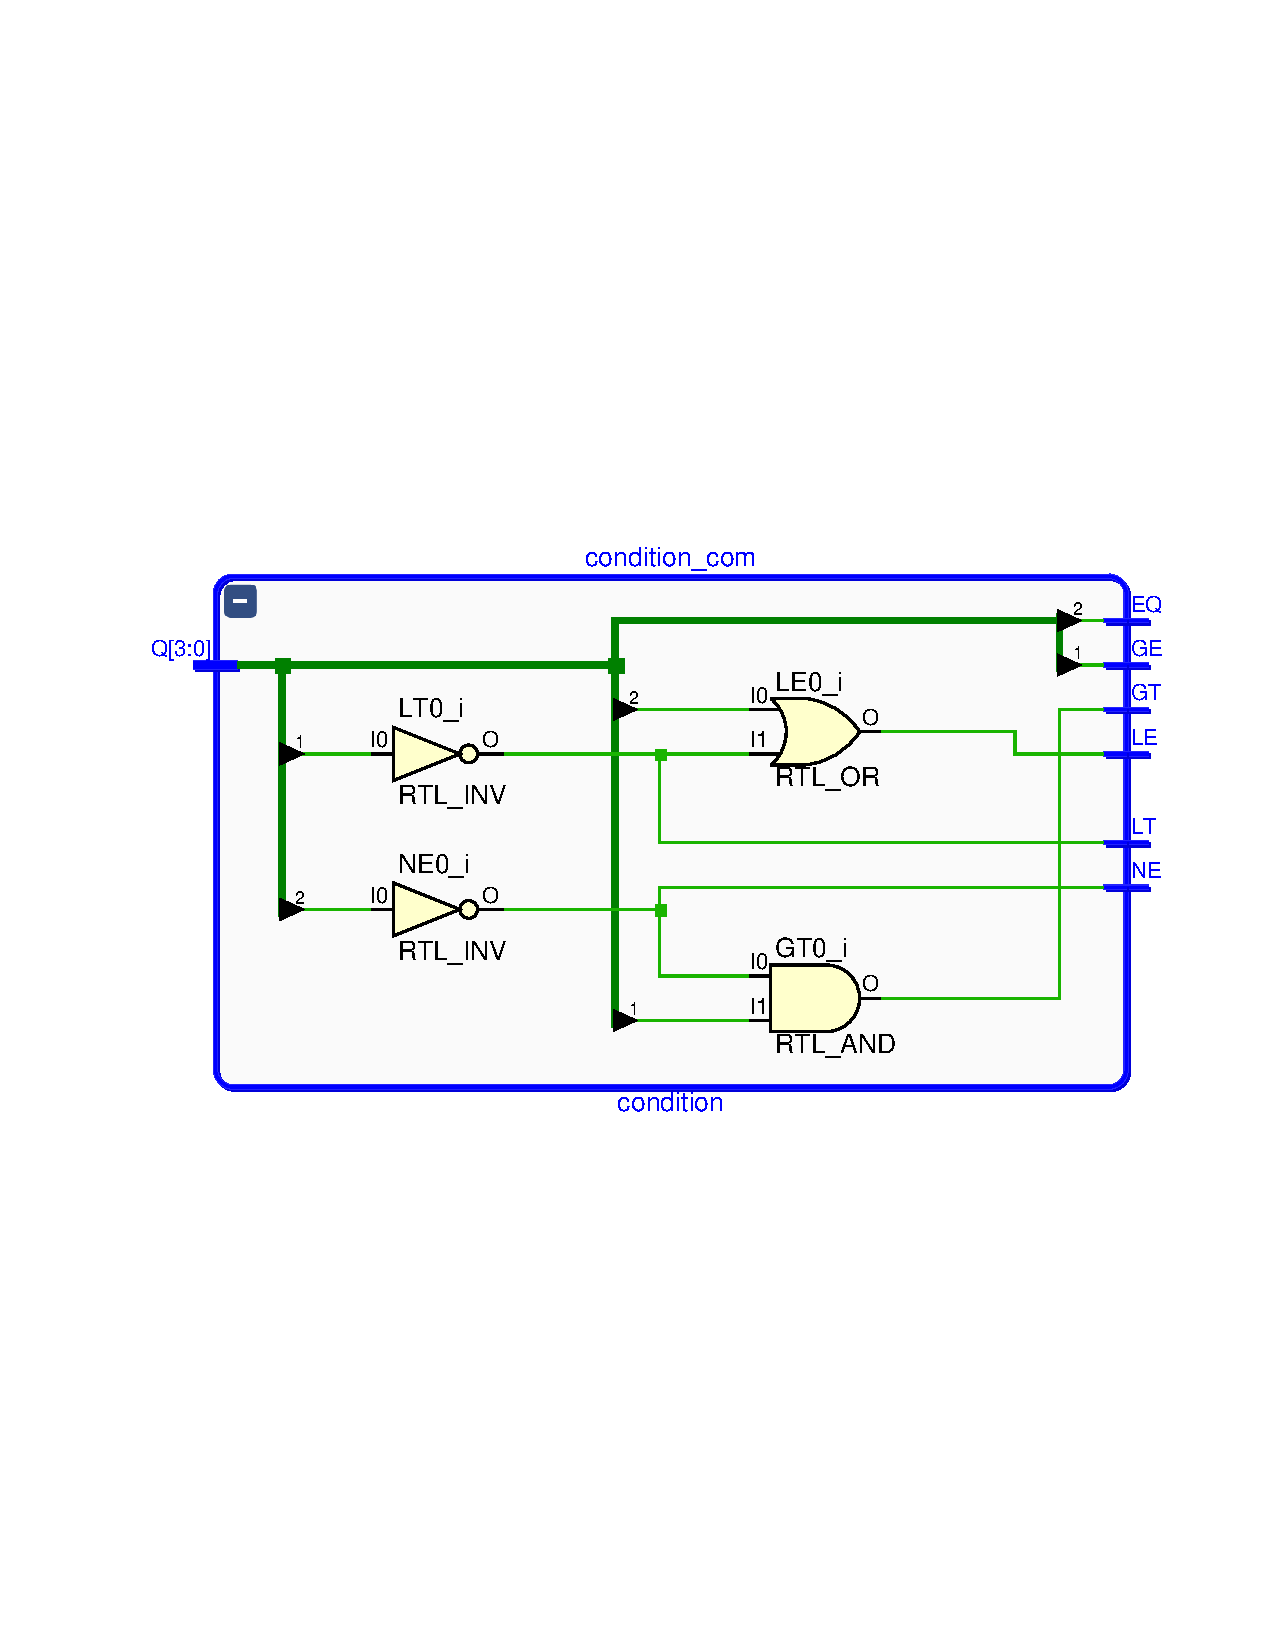
\includegraphics[scale=0.75]{rtl/condicion.pdf}
\end{center}
\subsection{Bloque decodificador}
\begin{center}
  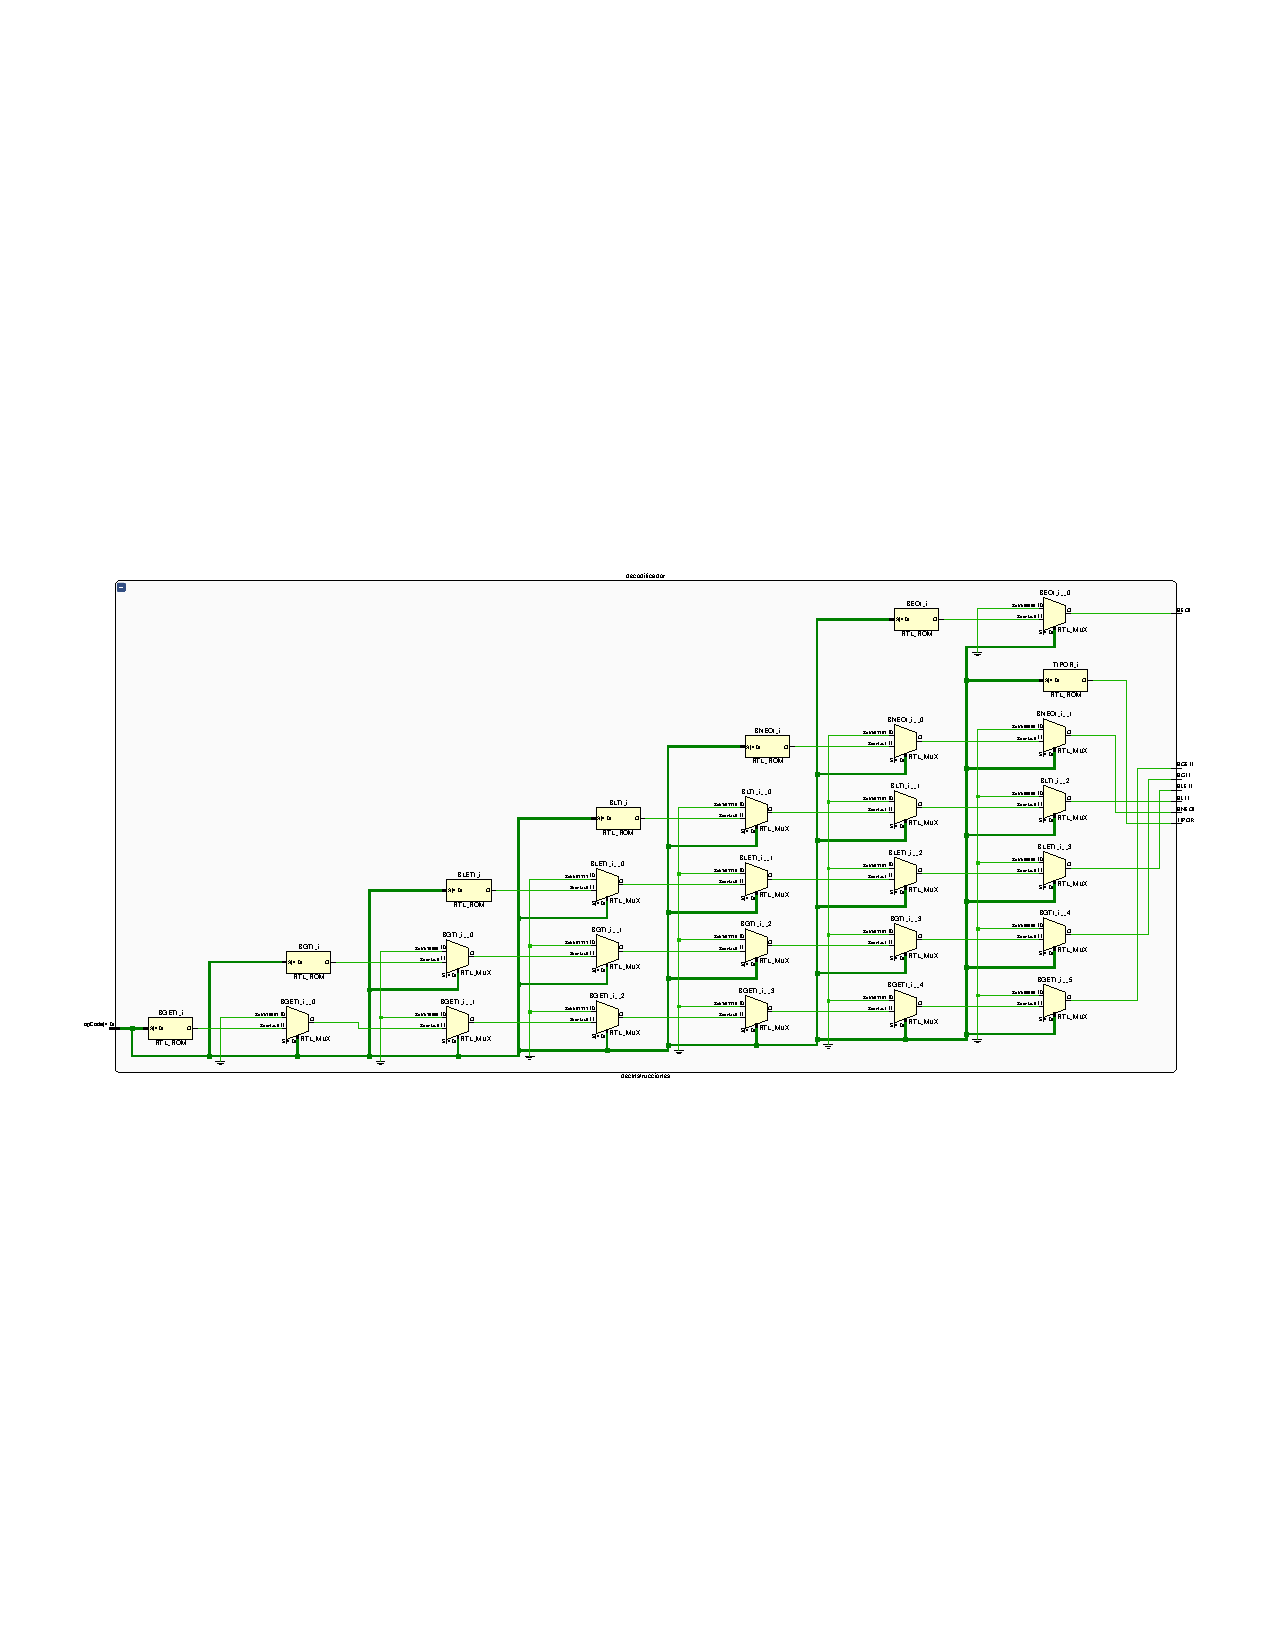
\includegraphics[scale=0.75]{rtl/deco.pdf}
\end{center}
\subsection{Bloque de nivel}
\begin{center}
  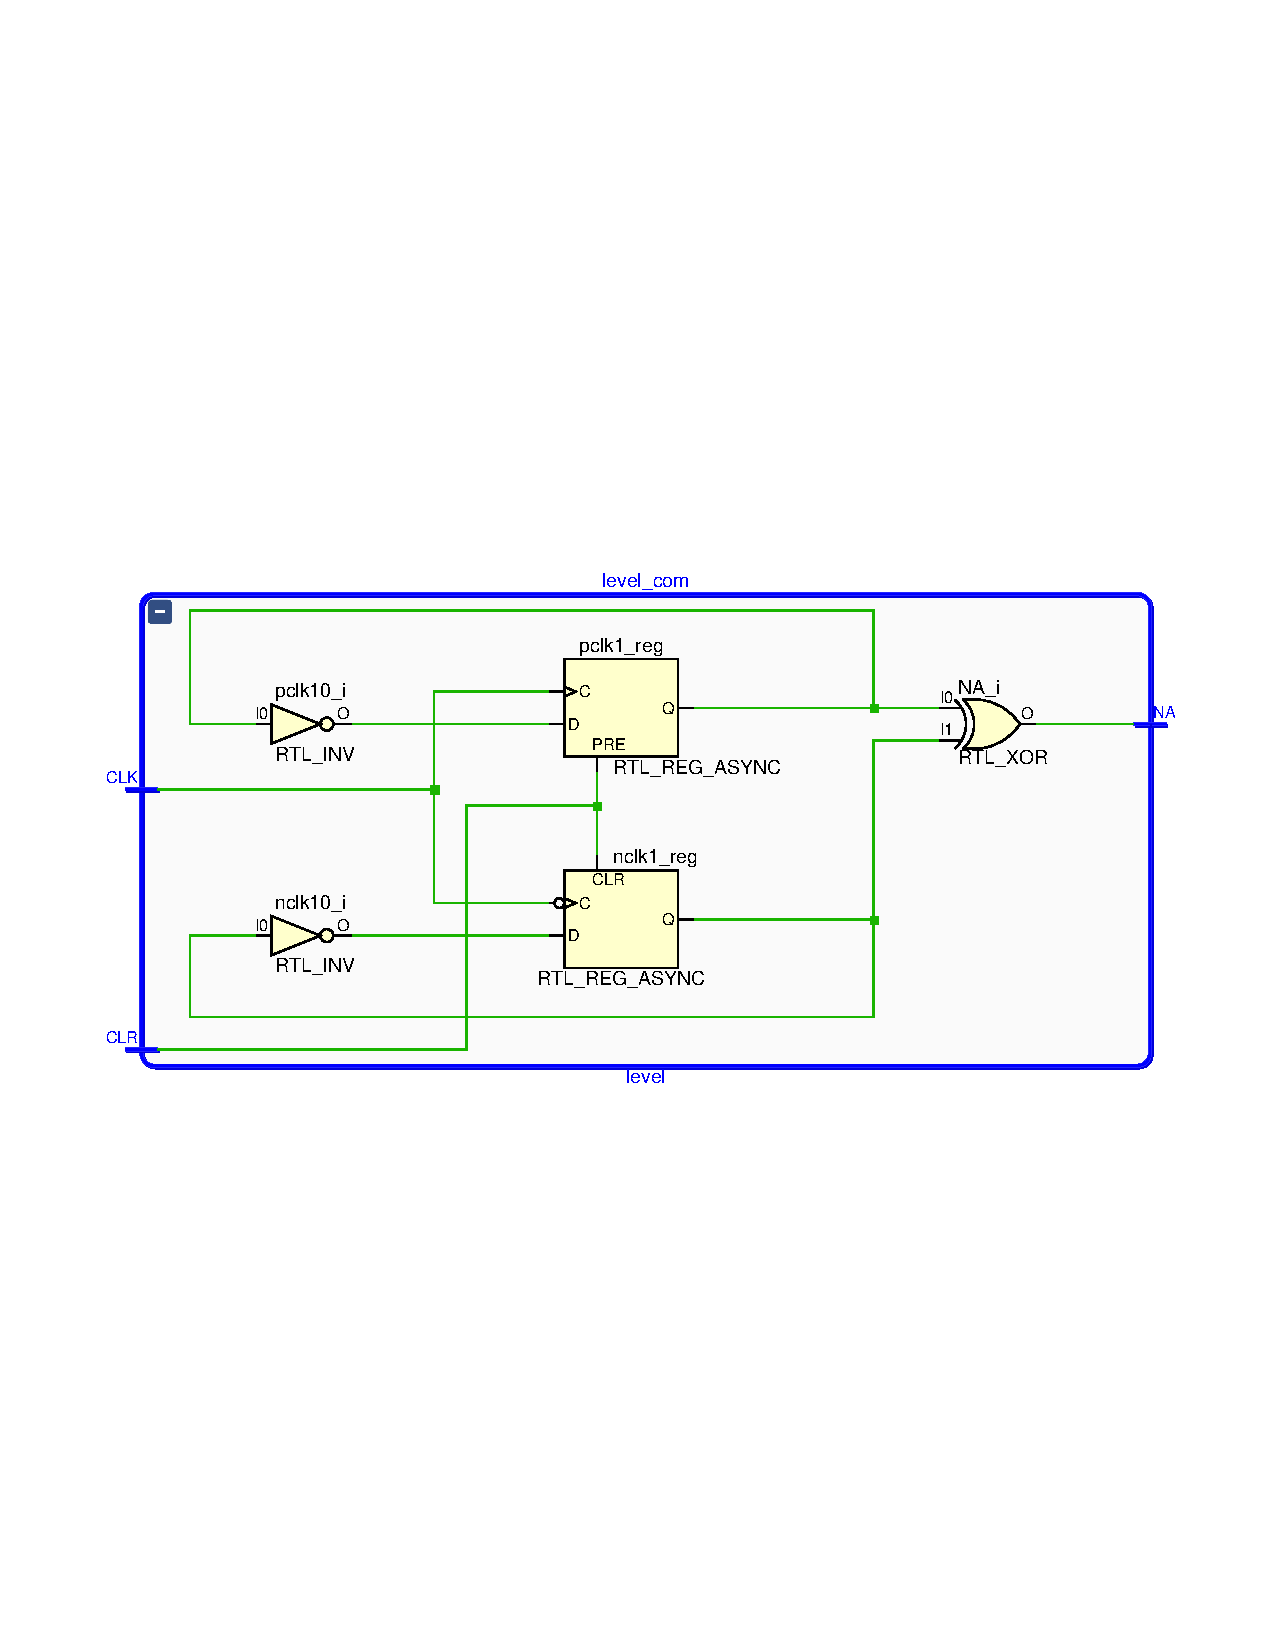
\includegraphics[scale=0.75]{rtl/nivel.pdf}
\end{center}
\subsection{MFunCode}
\begin{center}
  \includegraphics[scale=0.75]{rtl/mfuncode.pdf}
\end{center}
\subsection{MOpCode}
\begin{center}
  \includegraphics[scale=0.75]{rtl/mopcode.pdf}
\end{center}
\subsection{Unidad de Control}
\begin{center}
  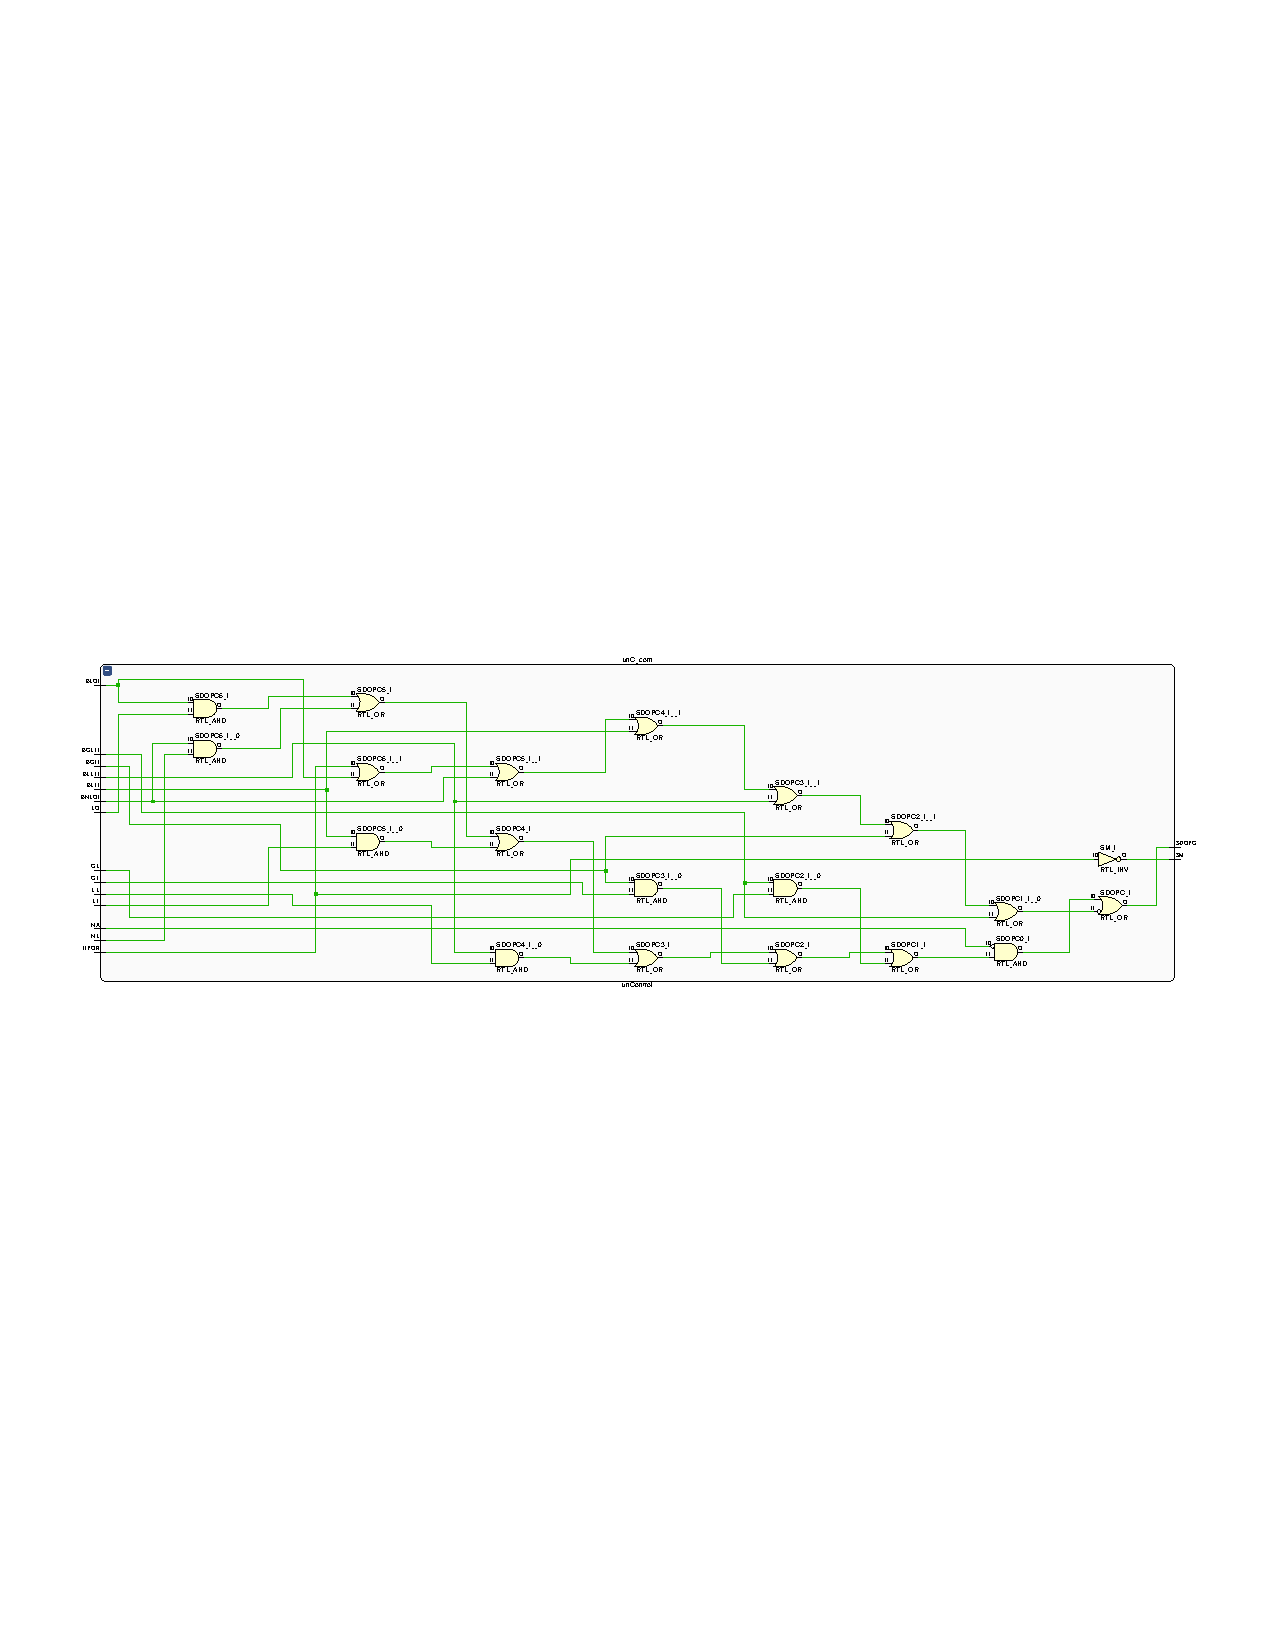
\includegraphics[scale=0.75]{rtl/control.pdf}
\end{center}
\subsection{Arquitectura completa}
\begin{center}
  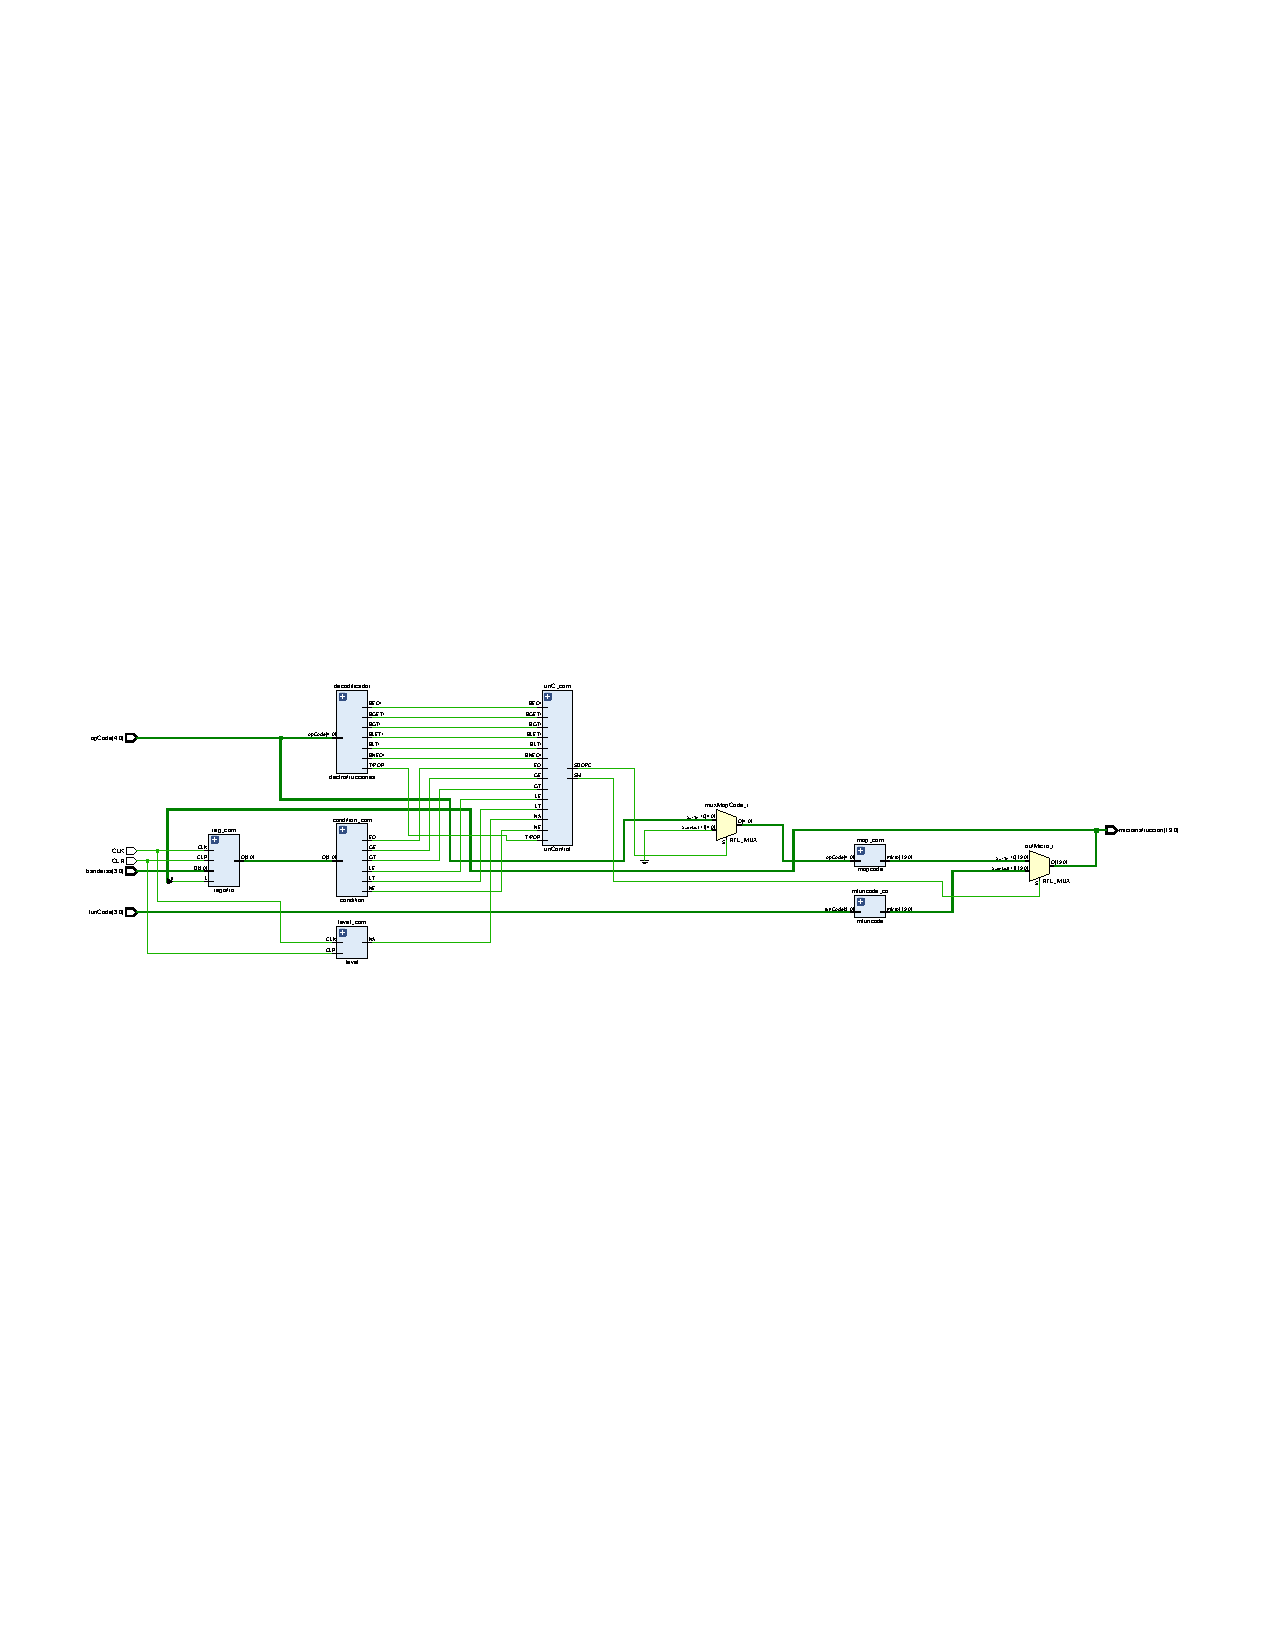
\includegraphics[scale=0.75]{rtl/arquitectura.pdf}
\end{center}

\end{document}
